\chapter{Data Acquisition System Usage}
\label{sect:systemUsage}
This section documents the steps required for correct usage of the data acquisition system.

\section{Integration}
The main data acquisition system should be integrated into the flight test vehicle near the vehicle's center of gravity.\nomenclature[A]{CG}{Center of gravity} The system should have one of its principal axes lined up roughly parallel to the vehicle's longitudinal axis. Servos should be connected to both the main board and the aircraft's receiver using a y-splitter with 2 male and one female connectors. If applicable, the servos should be connected according to the Table \ref{table:servoSetup}.
\begin{table}[ht]
\caption{Air Data System Setup}
\centering
\begin{tabular}{c c}
\hline\hline
 Servo & PWM Pinout\\
\hline
Throttle & D37\\
Elevator & D38\\
Rudder & D39\\ 
Aileron (1/2) & D40\\
Aileron (2/2) & D41\\
Gear & D42\\
Auxiliary (1/2)& D43\\
Auxiliary (2/2)& D44\\
\hline
\end{tabular}
\label{table:servoSetup}
\end{table}

If the additional digital pin-outs are being use for measuring servo signals, the ``+V'' jumper should not have a jumper on it. If using the digital pin-outs to run digital sensors or command servos, place the jumper on the appropriate voltage level setting.

The data acquisition system is powered through the barrel jack on the Arduino Due. The recommended operating voltage is between 7V and 12V, with an absolute maximum of 16V. The power can be supplied using either a battery dedicated to the data acquisition system, or through a BEC from the ESC. If using the ESC's BEC, set the BEC output somewhere between 7V and 12V. \textbf{CRITICAL:} ensure the red wire from the ESC does not pass to the receiver, as it is over-voltage for standard R/C equipment.\nomenclature[A]{ESC}{Electronic speed controller}\nomenclature[A]{BEC}{Battery elimination circuit}

The pressure board can be placed anywhere in the vehicle, as long as it can be connected to the main board. The pressure sensors should be attached to the five-hole probe as follows:

\begin{table}[ht]
\caption{Air Data System Setup}
\centering
\begin{tabular}{c c c c}
\hline\hline
 Pressure Sensor & Port A & Port B & Measurement\\
\hline
0 & Tube 5 & Tube 4 & $\beta$ \\
1 & Tube 6 & Tube 1 & $q_{\infty}$\\
2 & Tube 3 & Tube 2 & $\alpha$\\ 
3 & n/a & Tube 6 & $P_S$\\
\hline
\end{tabular}
\label{table:airDataSetup}
\end{table}
\nomenclature[A]{$P_S$}{Static pressure}

Port A and Port B refer to the ports as labeled in Figure \ref{fig:pressureLabels}, and the tube number refers to the five-hole probe tubes. These tube numbers increase as the tube length decreases: Tube 1 refers to the longest tube, Tube 6 refers to the shortest tube.

\begin{figure}[H]
  \centering
    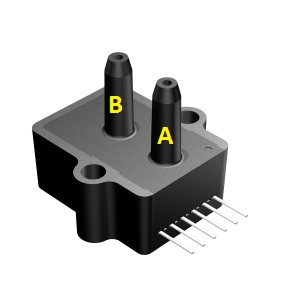
\includegraphics[width=0.5\textwidth]{figures/allsensorsPressureLabeled.jpg}
      \caption{Port Description for Pressure Sensors} \label{fig:pressureLabels}
\end{figure}

The pressure tubing and temperature sensor line should be routed together to the air data boom and secured for flight. The temperature sensor's wiring is a standard servo extension. The air data boom's accelerometer wiring is a standard RJ-25 \textit{patch} cable and should be routed in a separate bundle, as it will be removed before flight.

The air data boom itself should be integrated as far from aerodynamic effects as possible. For this thesis, the boom was mounted roughly one chord length in front of the leading edge of the wing and approximately halfway down the wing span. Other mounting locations could include out the aircraft's nose for a pusher vehicle, or on the vertical tail. The aluminum block accepts a 0.25" carbon fiber tube as it's mounting interface, and this tube should be mounted roughly in-line with the airflow angle expected during flight. The temperature sensor can be taped to the tube.

\section{Pre-flight Procedure}
\label{sect:preFlightProc}
The pre-flight procedure in this section must be completed in addition to all preparation listed in Section \ref{sect:flightTestProc}.

\begin{enumerate}
\item With the transmitter turned on, power on the receiver.
\item Plug in the micro-USB cable into the main data acquisition board.
\item Ensure the micro-SD card is empty and formatted as FAT32, then insert it into the main data acquisition board.
\item Plug in the main data acquisition system's battery pack or the BEC. \textbf{CRITICAL:} ensure the red wire does not connect the BEC to the receiver.
\item Plug the pressure sensor board into the main data acquisition board.
\item Plug in the air data system's RJ-25.
\item Upload the calibration routine to the main board, and follow the prompts to calibrate the gyroscope, accelerometer, and magnetometers.
\item Place a wind blocker (Daisy/Solo cups work) over the five-hole probe and calibrate the pressure sensors, using the calibration routine.
\item Load the main data acquisition script onto the main data acquisition board.
\item Turn on serial output and check that all sensors are functioning properly.
\item Initialize the micro-SD card.
\item Turn off serial output.
\item Turn on data logging and verify the system is saving data.
\item Remove the micro-USB cable and the air data system's RJ-25 cable.
\item Plug in the main propulsion battery pack.
\end{enumerate}
The data acquisition system is now ready for flight.

\section{Flight test plan}
When using the data acquisition system for drag polar estimation, a better model estimate is possible with proper flight maneuvers. The main technique to improve the model is to vary speeds as much as possible, which allows more of the drag polar to be flown. Multiple glides that begin at the highest speed possible should be completed. To achieve the highest initial gliding speed, the aircraft should be put into a dive at full throttle, with plenty of available altitude. Throttle should then be cut, and the dive should briefly continue. After a few seconds of diving, the aircraft should be leveled off and altitude should be maintained, until the vehicle stalls. Repeating this process will provide a large sweep of the flight envelope.

Inverted flight can also help fill out the section of the drag polar that occurs below $C_{L_{min}}$. However, inverted flight should occur at high speeds, to avoid the nonlinear section of the inverted airfoil.

\section{Post-Flight}
Immediately after the vehicle lands, the vehicle's propulsion pack should be unplugged. Next, unplug the data acquisition system's battery pack, remove the micro-SD card, and save the data to a computer. Optionally, after the flight is complete, a second round of zero offset calibration data may be acquired. This set ensures that any drift that occurred during the flight is accounted for.

Once the data is saved to a computer, the data analysis GUI can be used to quickly process the data. \nomenclature[A]{GUI}{Graphical user interface} The user interface can estimate a drag polar using the following steps:
\begin{enumerate}
\item Run \texttt{fileReader.m}.
\item Click the ``Load Data'' button to load flight data. If you'd like an ASCII data file, choose yes on the prompt.
\item Select the pressure calibration file.
\item Select the accelerometer/gyroscope calibration file.
\item Select the magnetometer calibration file.
\item Select the air data system alignment calibration file.
\item Input the reference area in the $S_{REF}$ box and the weight in the Weight box.
\item Click ``Ignore Data With Thrust.''
\item Click ``Display'' in the Quadratic Fit box.
\end{enumerate}

Google Earth plots are also available by clicking the ``Google Earth'' button. The ``X Axis'' and ``Y Axis'' drop down menus are also available, which allows any signal to be plotted against any other signal.

\section{Embedded Software Protocol}
The main data acquisition code allows the user to interface with the Arduino through a serial text interface. A list of available commands for the main data acquisition script, along with their intended functions, is shown in Table \ref{table:mainScriptComms}.
\begin{table}[H]
\caption{Available Commands for \texttt{mainScript.ino}}
\centering
\begin{tabular}{|c | c|}
\hline
 Command & Utility\\
 \hline\hline
dataOn & Turn on data logging to SD card\\\hline
dataOff & Turn off data logging to SD card\\\hline
initSD & Initialize SD card\\\hline
serialOn & Turn on serial output\\\hline
serialOff & Turn off serial output\\\hline
? & Help menu\\\hline
\end{tabular}
\label{table:mainScriptComms}
\end{table}

Note that all commands must be sent with a start character (`\texttt{\#}') and an end character (`\texttt{\&}'.) A proper command to turn on serial output would then be \texttt{`\#serialOn\&'}.

The calibration code also interfaces with the Arduino using a text interface. The calibration script's commands are shown in Table \ref{table:calibComms}.
\begin{table}[H]
\caption{Available Commands for \texttt{calibration.ino}}
\centering
\begin{tabular}{|c | c|}
\hline
 Command & Utility\\
 \hline\hline
accelGyro & Calibrate accel for slope and offset, gyro for offset, and probe alignment. 
Saved to \texttt{ACCLGYRO.clb}.\\\hline
pressure & Calibrate offset of pressure sensors. 
Saved to \texttt{PRESSURE.clb}.\\\hline
mag & Calibrate magnetometers for hard- and soft-iron effects. 
Saved to \texttt{MGNTMTRS.clb}.\\\hline
? & Help menu\\\hline
\end{tabular}
\label{table:calibComms}
\end{table}

Note that, like the main script, all commands must be sent with a start character (`\texttt{\#}') and an end character (`\texttt{\&}'.) A proper command to calibrate the air data system alignment would then be \texttt{`\#pressure\&'}.